\section{MARCO TECNOLÓGICO}

El problema que se busca solucionar en este trabajo tiene relación directa con el estudio de la visión por ordenador. Este campo de la Ingeniería busca, 
a través de sistemas de captación y procesamiento de imágenes, generar información y automatizar procesos con ordenadores. \newline Dentro de este área se han desarrollado tecnologías que usamos día a día
\cite{szeliskiComputerVisionAlgorithms2022}:

\begin{itemize}
    \item \textbf{\textit{\acrfullr{ocr}}} para realizar reconocimiento de texto en imágenes y documentos.
    \item \textbf{Detección de fallos en maquinaria} en procesos de fabricación.
    \item \textbf{Fotogrametría} para mapear imágenes a modelos \texttt{3D}.
    \item \textbf{Imagen médica} para uso en operaciones a tiempo real\cite{NEMESIS3DCM}.
    \item \textbf{Detección de objetos} en imágenes o videos.
    \item \textbf{Detección de movimiento} y seguimiento de objetos en escenas.
\end{itemize}

Las aplicaciones que usan herramientas basadas en este tipo de soluciones suelen seguir una estructura similar a la siguiente:

\begin{enumerate}
    \item Capturar información a través de cámaras o flujos de video IP de diferentes características.
    \item (A veces) Realizar un preprocesamiento de las imágenes para adaptarlas al sistema.
    \item Procesar las imágenes para extraer información relevante para el sistema.
    \item Transformar la información extraída a través de algoritmos inteligentes para construir una base de datos que sea útil para el usuario de la aplicación.
\end{enumerate}

En el caso de este trabajo, se tratan problemas de detección de objetos y análisis de cambio. Este tipo de tareas se han llevado a cabo antiguamente a través de algoritmos complejos y deterministas, pero en los últimos 
años, con el auge del aprendizaje automático, se ha creado un nuevo paradigma.

En los siguientes puntos se van a describir de forma breve las técnicas de aprendizaje automático, los sistemas de detección de objetos, seguimiento de cambio y los entornos de desarrollo y despliegue 
de estas técnicas de forma transparente al \texttt{Hardware} disponible así como proyectos relacionados con este trabajo.
\clearpage

\subsection{Aprendizaje Automático y \texttt{Deep Learning}}

\subsubsection{Definición y tipos de tareas}

El campo del aprendizaje automático busca desarrollar soluciones a través de algoritmos y sistemas que permitan a los ordenadores tratar los datos entrantes como el cerebro humano, siendo capaz de 
generalizar las propiedades que les definen y encontrar patrones.

Este aprendizaje automático se realiza sobre un conjunto de datos que aporta el usuario con el objetivo de abstraer diferentes informaciones específicas o agrupar los datos según patrones. Este aprendizaje 
habitualmente se realiza a través de un bucle de tres fases (ver \autoref{fig:FasesAprendizaje}) en las cuales se configura el sistema para aprender, se valida el sistema resultante y se reconfiguran los parámetros para acercarse a un sistema 
que aporte mejores resultados.

\begin{figure}[H]
    \centering
    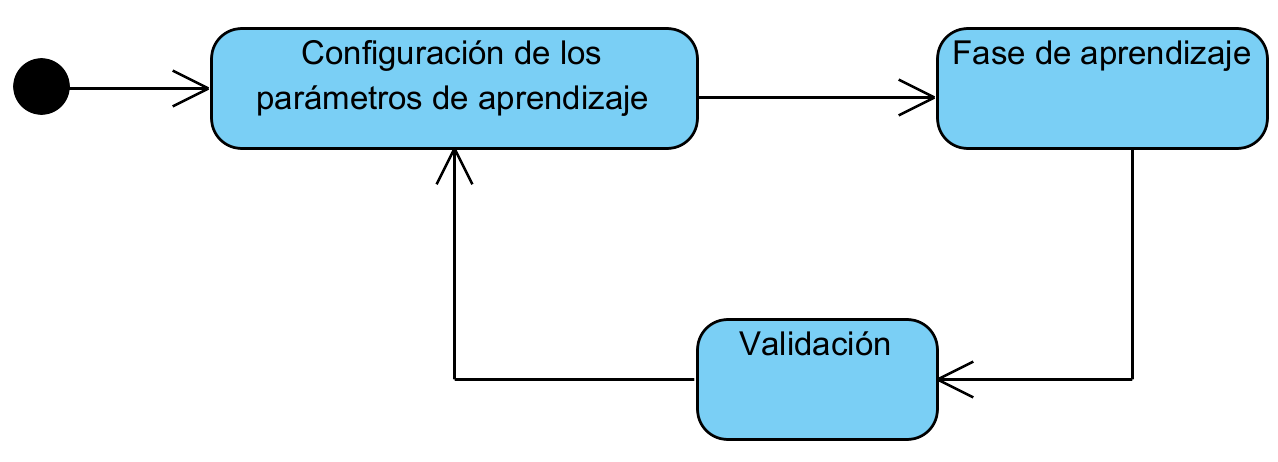
\includegraphics[width=0.7\textwidth]{images/4/Fases.png}
    \caption{Bucle de fases de aprendizaje en un sistema de \texttt{Machine Learning}}
    \label{fig:FasesAprendizaje}
\end{figure}

Dentro del campo existen diferentes ramas dependientes del objetivo del aprendizaje que se busca y los datos con los que vamos a alimentar el sistema:

\begin{itemize}
    \item \textbf{Entrenamiento supervisado}: es un tipo de entrenamiento en el que se conoce la relación entre los datos de entrada y los datos esperados. 
    \item \textbf{Entrenamiento no supervisado}: el objetivo de este aprendizaje es aprender las relaciones de los datos de entrada entre sí.
    \item \textbf{Entrenamiento reforzado}: es una variación del entrenamiento supervisado en el que el sistema recibe feedback sobre los resultados como parte de la fase de aprendizaje. Se utiliza 
    mucho en el ámbito de la robótica.
\end{itemize}

Entre todas las técnicas que implementan este tipo de tareas, uno de los sistemas modernos más conocidos son las redes neuronales.

\subsubsection{Redes Neuronales}

Este campo tiene su origen en una publicación de Warren McCulloch y Walter Pitts en 1943\cite{mccullochLOGICALCALCULUSIDEAS} en el que presentaban la idea de neurona como una unidad lógica básica 
implementable cuyo estado se puede definir como un "todo o nada", lo cual se representa en el campo de las telecomunicaciones con una función escalón como se ve en la \autoref{fig:Escalon}. Este 
trabajo y diseño de neurona sería conocido más tarde como perceptron.

\begin{figure}[H]
    \centering
    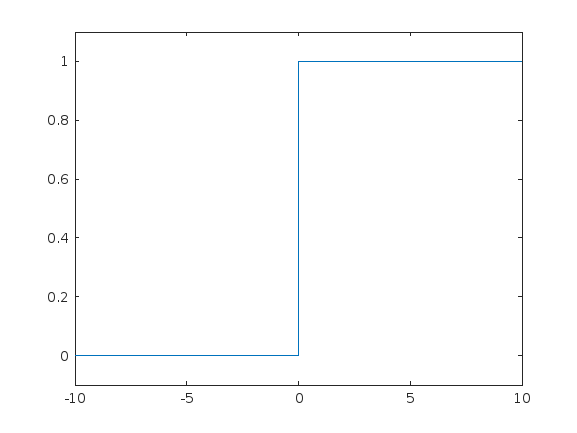
\includegraphics[width=0.3\textwidth]{images/4/Escalon.png}
    \caption{Figura de activación escalón de las primeras neuronas}
    \label{fig:Escalon}
\end{figure}

La estructura básica del perceptron se puede observar en la \autoref{fig:Perceptron} y consiste en un nodo con un número \(\mathcal{N}\) de conexiones entrantes, con un peso asociado \(\mathcal{W}\) 
a cada entrada. El nodo calcula el sumatorio de cada conexión con su respectivo peso. Al resultado de este cálculo se le añade un factor de \texttt{bias} y por último, mediante una función de 
activación como la vista anteriormente, se decide el resultado de salida de la neurona. 

\begin{figure}[H]
    \centering
    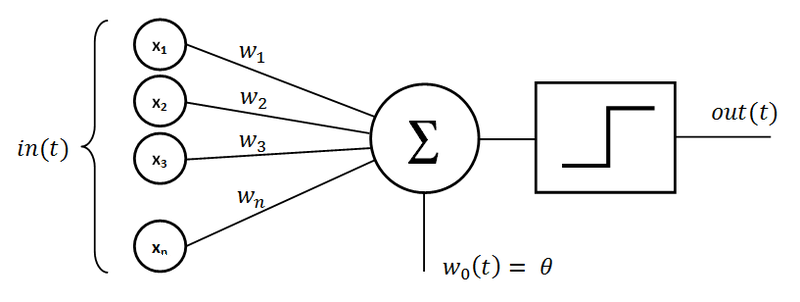
\includegraphics[width=0.5\textwidth]{images/4/perceptron.png}
    \caption{Diagrama general de un perceptron\cite{JgfisherPerceptronPerceptron}}
    \label{fig:Perceptron}
\end{figure}

Más tarde, se conseguiría implementar un diseño electrónico de esta neurona, e interconectar más neuronas entre sí. Estas interconexiones dan lugar a la creación del concepto de \textbf{redes neuronales}, 
siendo una de las primeras redes complejas funcionales de tipo \texttt{\acrfullr{mlp}}. Estos sistemas serían clave para la evolución del aprendizaje automático, apareciendo multitud de 
variaciones en la arquitectura de la red según las necesidades (ver \autoref{fig:ArquitecturasRedes}).

\begin{figure}[H]
    \centering
    \begin{subfigure}[b]{0.25\textwidth}
        \centering
        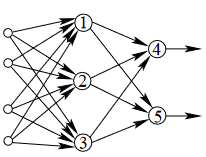
\includegraphics[width=0.9\textwidth]{images/4/FeedForward.png}
        \caption{Red FeedForward}
        \label{fig:a}
    \end{subfigure}
    \begin{subfigure}[b]{0.25\textwidth}
        \centering
        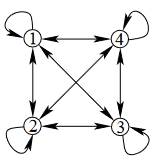
\includegraphics[width=0.7\textwidth]{images/4/Recursiva.png}
        \caption{Red recursiva}
        \label{fig:b}
    \end{subfigure}
    \begin{subfigure}[b]{0.45\textwidth}
        \centering
        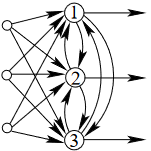
\includegraphics[width=0.4\textwidth]{images/4/FeedForwardLateral.png}
        \caption{Red FeedForward con inhibidores laterales}
        \label{fig:c}
    \end{subfigure}
    \caption{Diferentes ejemplos de arquitecturas simples de redes neuronales\cite{duNeuralNetworksStatistical2013}}
    \label{fig:ArquitecturasRedes}
\end{figure}

El avance progresivo de la capacidad de cómputo de los ordenadores ha permitido el uso de redes neuronales de mayor tamaño, que permiten mayor capacidad de abstracción. Es en este marco donde aparece el término 
\texttt{Deep Learning}, que no indica nada más que el uso de redes neuronales con una cantidad masiva de capas intermedias. Además, son sistemas que trabajan muy bien cuando se implementan con ejecución paralela, 
aunque esto se explicará más adelante.

Este tipo de sistemas han demostrado su gran capacidad de abstracción y rapidez, es por esto mismo que las redes neuronales profundas son una de las principales herramientas que se utilizan hoy en día en 
visión por ordenador.

\clearpage
\subsection{Detección de Objetos con redes neuronales}

La detección de objetos como tarea surge de la necesidad de analizar la existencia de objetos en imágenes y; opcionalmente, localizarlos en las mismas. Para realizar este tipo de tareas se han ido 
desarrollando técnicas tradicionales basadas en algoritmos deterministas, pero, con el auge del aprendizaje automático, a partir de 2012\cite{zouObjectDetection202023} 
el paradigma pasó a centrarse en la creación de sistemas detectores basados en \texttt{Deep Learning} (Sistemas de Redes Neuronales con una gran cantidad de capas ocultas).

Ambas técnicas se basan en la extracción y el análisis de características de las imágenes, esto es, la caracterización de imágenes o zonas de interés a través de algoritmos o filtros. Podemos entender la caracterización 
de una imagen como la parametrización de los elementos que la definen. Dentro de la vista humana existen muchos elementos que se pueden usar para definir una imagen, algunos ejemplos son:
\begin{itemize}
    \item \textbf{Nitidez}.
    \item \textbf{Color}.
    \item \textbf{Presencia de ciertas formas geométricas}.
    \item \textbf{Brillo}.
    \item \textbf{Ruido}
\end{itemize}

Se debe tener en cuenta que estos ejemplos son características que da un humano para una imagen, de forma contraria, las redes neuronales trabajan con características de bajo nivel (P. ej.: existencia de bordes en una zona específica, colores en un área, 
patrones de puntos, etc.) que permitan analizar zonas de la imagen. Sin embargo, las redes neuronales tipo \texttt{\acrshort{mlp}} no fueron pensadas para este tipo de tareas. Esto es debido a que el 
análisis de características en una imagen es una tarea cuya dificultad computacional aumenta de forma exponencial con el aumento de la resolución, ya que, para cualquier imagen, debería haber una neurona de entrada por 
cada pixel y canal de la imagen, sobre cuyos valores la red \texttt{\acrshort{mlp}} aplicaría los cálculos.

Por estos motivos, se buscó una forma de añadir independencia espacial a la entrada de las redes neuronales. Esto se consigue mediante el uso de diferentes arquitecturas, siendo la más importante las redes 
neuronales convolucionales.\newline

\subsubsection{Arquitecturas de redes neuronales tipo \texttt{CNN}}

Las \texttt{\acrfullr{cnn}} definen una arquitectura basada en dos pasos: la extracción de las características de las imágenes y la clasificación de las imágenes según las características. Su estructura básica se 
puede ver \autoref{fig:ArquitecturaCNN} y  se compone de dos subredes que cumplen las dos funciones diferentes para los datos de entrada.

\begin{figure}[H]
    \centering
    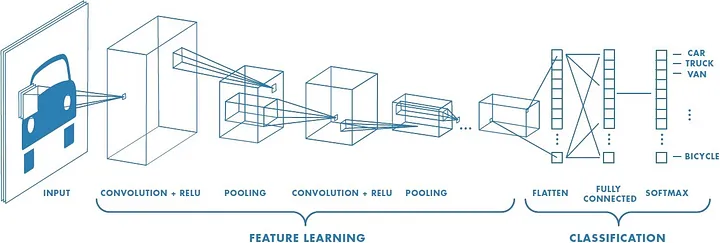
\includegraphics[width=0.9\textwidth]{images/4/ArquitecturaCNN.png}
    \caption{Arquitectura básica de una \texttt{CNN}\cite{sahaComprehensiveGuideConvolutional2022}}
    \label{fig:ArquitecturaCNN}
\end{figure}

\clearpage

La fase de caracterización se compone principalmente de capas neuronales convolucionales y, habitualmente capas de \texttt{pooling}:

\begin{itemize}
    \item Capas convolucionales: tienen como objetivo la extracción de características a través de neuronas que implementan operaciones de convolución sobre las imágenes. 
    Al ser las imágenes tensores, se les aplican filtros convolucionales implementados a través de \texttt{Kernels}. 
    Dependiendo de la característica a buscar, existen diferentes filtros convolucionales y en las fases de entrenamiento se va conformando el \texttt{Kernel} que caracteriza mejor esa zona de la imagen para los datos esperados.

    Un ejemplo de \texttt{Kernel} es un filtro laplaciano gaussiano como el de la \autoref{fig:LaplaceKernel}, que, a través del gradiente, sirve para darle más énfasis a los bordes de la imagen, como se puede ver 
    en la \autoref{fig:LaplaceResultado}.
    \begin{figure}[H]
        \centering
        \(
        \begin{vmatrix}
            1 & 1 & 1 \\
            1 & -8 & 1 \\
            1 & 1 & 1
        \end{vmatrix}
        \)
        \caption{Aspecto de un \texttt{kernel} de Laplace de tamaño \texttt{3x3}}
        \label{fig:LaplaceKernel}
    \end{figure}
    \begin{figure}[H]
        \centering
        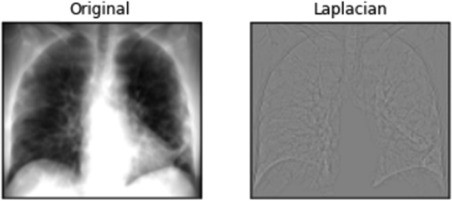
\includegraphics[width=0.7\textwidth]{images/4/KernelsTipicos.jpg}
        \caption{Aplicación de un filtro gaussiano de Laplace a una imagen médica\cite{LaplacianFilterOverview}}
        \label{fig:LaplaceResultado}
    \end{figure}

    Estas capas convolucionales van obteniendo la abstracción de las características transformando los volúmenes de entrada a volúmenes de salida de mayor profundidad pero de menor resolución vertical y horizontal.\newline
    Habitualmente en la parte convolucional se utilizan funciones de activación como la \acrfullr{relu} de la \autoref{fig:relu}.
    \begin{figure}[H]
        \centering
        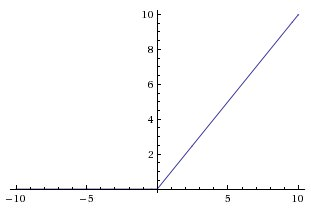
\includegraphics[width=0.5\textwidth]{images/4/relu.jpeg}
        \caption{Función de activación \texttt{ReLU}}
        \label{fig:relu}
    \end{figure}
    \clearpage
    \item Capas de \texttt{pooling}: Su objetivo es ir haciendo sub-muestreo de las capas convolucionales superiores para conformar el volumen de entrada de la siguiente capa convolucional, reduciendo la carga computacional necesaria. 
    Se puede ver su funcionamiento en la \autoref{fig:MuestreoCNN}, donde sub-muestrean un volumen de resolución \texttt{28x28} a una resolución \texttt{14x14}, pero habitualmente se aumenta la profundidad del tensor.
    \begin{figure}[H]
        \centering
        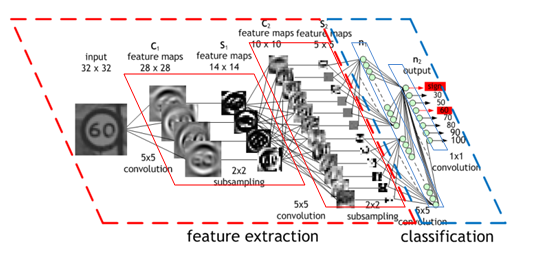
\includegraphics[width=0.6\textwidth]{images/4/EjemploPolling.png}
        \caption{\texttt{CNN} con detalle de la caracterización y el sub-muestreo\cite{ConvolutionalNeuralNetwork}}
        \label{fig:MuestreoCNN}
    \end{figure}
    
    Este sistema se va repitiendo para cada capa de convolución, hasta que en la última capa de \texttt{pooling}, la salida es un vector horizontal cuyo tamaño es el miso que neuronas de entrada tenga la etapa de clasificación. 

\end{itemize}


La fase de clasificación habitualmente se compone de una capa conectada completamente como se ha podido ver en la anterior sección, similar a la idea de una \texttt{\acrshort{mlp}}. Esta 
red toma como entrada un vector aplanado final de la parte de extracción de características y realiza la clasificación. Habitualmente utiliza funciones de activación que son capaces de tener \(\mathcal{N}\) salidas 
una de estas funciones habituales es la \texttt{SoftMax} de la \autoref{fig:softmax}, que mapea un vector de entrada a un vector de salida de probabilidades que escalan según los valores de entrada.

\begin{figure}[H]
    \centering
    \begin{equation*}
        \text{softmax}(z_i) = \frac{e^{z_i}}{\sum_j e^{z_j}}
    \end{equation*}
    \caption{Función de activación \texttt{SoftMax}}
    \label{fig:softmax}
\end{figure}

\vspace{3\baselineskip}

El uso de estas redes neuronales convolucionales para solucionar un problema está asociado al tipo de trabajo a realizar. Cuando se define un problema en el que se va a aplicar esta técnica, normalmente 
cae en tres tipos de categorías presentadas en la \autoref{fig:tareasCNN}. Además, esta selección tiene unas implicaciones en la complejidad computacional de la tarea, ya que la capa de clasificación debe ser cambiada para soportarla.

\begin{itemize}
    \item Clasificación: las imágenes son marcadas dependiendo de si existe o no un elemento específico dentro de ella.
    \item Detección de objetos: regiones locales de la imagen son clasificadas y marcadas dependiendo de la existencia del elemento en cuestión.
    \item Segmentación semántica: se realiza una clasificación por cada pixel para delimitar todos los píxeles que conforman la instancia del objeto.
\end{itemize}

\begin{figure}[H]
    \centering
    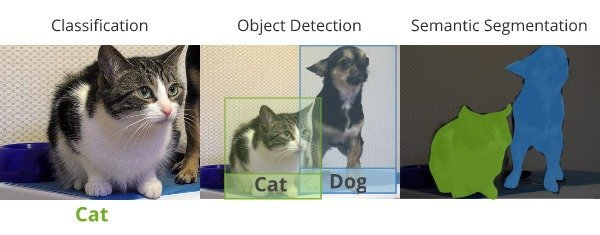
\includegraphics[width=0.6\textwidth]{images/4/TiposTareas.png}
    \caption{Tareas típicas de una \texttt{CNN}\cite{kallfelzsirmacekSEQUENTIALIMAGEPROCESSING2019}}
    \label{fig:tareasCNN}
\end{figure}

Toda red neuronal sobre la que se realice entrenamiento supervisado debe ser entrenada con un conjunto de datos etiquetados de forma coherente a la tarea que se quiera realizar. Por ejemplo, una \texttt{CNN} 
entrenada para clasificar imágenes deberá ser alimentada con etiquetas adecuadas, no con coordenadas sobre la posición del elemento detectado.

Estos conjuntos de datos que se preparan para las redes neuronales se dividen habitualmente en conjuntos con diferentes propósitos en el entrenamiento de la red neuronal:

\begin{itemize}
    \item Conjunto de datos de entrenamiento: es el conjunto de datos sobre el que la red va a aprender, aplicando de forma constante su algoritmo. Pasar por este conjunto entero una vez suele llamarse época 
    de entrenamiento.
    \item Conjunto de datos de prueba: es un conjunto de datos completamente separado que nunca se aplicará a la red en la fase de entrenamiento. Su objetivo es evaluar al final del entrenamiento el 
    rendimiento general de la red en un conjunto de datos que nunca haya visto.
    \item Conjunto de datos de validación: estos datos se utilizan como conjunto de referencia entre épocas, su existencia y uso depende de la arquitectura de red neuronal, ya que existen 
    algunos algoritmos que modifican parámetros del entrenamiento de la red entre épocas.\newline
    Cuando se habla de los parámetros de la red, habitualmente se refieren a cosas como los pesos entre neuronas, la función de activación, el número de capas ocultas, etc\dots Sin embargo, los parámetros 
    que se definen para el entrenamiento como el número de épocas, parámetros del algoritmo de aprendizaje, tamaño de los datos introducidos a la vez, etc., son llamados hiperparámetros.
\end{itemize}

Normalmente se dispone de un conjunto de datos que se divide en entrenamiento, validación y prueba. Es habitual una separación de \texttt{70\%} para el conjunto de entrenamiento, \texttt{15\%} para el conjunto de 
validación y \texttt{15\%} para el conjunto de prueba.

La incorrecta preparación del conjunto de datos puede afectar severamente a los resultados obtenidos. Por lo tanto es habitual intentar evitar redundancia de datos y alimentar a la red con datos que no sean muy 
similares entre sí para que sea capaz de generalizar correctamente en la mayor cantidad de situaciones posibles.

Para solucionar este problema, podemos encontrar técnicas de aumento de datos, que generan artificialmente datos extra haciendo transformaciones en las imágenes, cambiando el color o incluso aplicando distorsión. 
Esto permite solucionar situaciones en las que se dispongan de pocos datos o los datos sean demasiado parecidos entre sí como para poder asegurar una buena generalización a otros tipos de situaciones.

\clearpage

La evolución de estas \texttt{\acrshort{cnn}} ha sido exponencial y han aparecido arquitecturas que han ido añadiendo mejoras de eficiencia, calidad de resultados y estándares a la hora de crear nuevos 
sistemas. Algunos ejemplos de esto son:
\begin{itemize}
    \item \texttt{R-CNN (Region-CNN)}(2014): introdujo el análisis solo en regiones con datos interesantes.
    \item \texttt{Fast R-CNN} (2015): mejora R-CNN introduciendo búsqueda selectiva, definiendo un número máximo de \texttt{\acrfullr{roi}} a tratar.
    \item \texttt{Faster R-CNN} (2015).
    \item \texttt{\acrfullr{yolo}}\cite{redmonYouOnlyLook2016}: arquitectura extremadamente rápida perteneciente al estado del arte moderno en redes neuronales, que ha ido mejorándose en forma de versiones.
\end{itemize}

Cada arquitectura ha traído consigo mejoras, a veces, a cambio de perdida de rendimiento. Esto es un problema que debe tenerse en cuenta y existen diversos trabajos que tratan simplemente las diferencias 
existentes entre diferentes arquitecturas.

Uno de estos trabajos\cite{hanAdvancedDeepLearningTechniques2018} compara diferentes arquitecturas contra el conjunto de datos de la universidad de Oxford "Pascal2012"\cite{PASCALVisualObject}, que contiene 20 clases de objetos. 

A través del estudio del estado del arte realizado en el artículo, se observa que \texttt{YOLOv2} es muy competente a la hora de obtener rendimiento y velocidad de procesamiento, aún sin ser la red con los mejores resultados, es 
capaz de superar a arquitecturas ya establecidas como \texttt{SSD512}, obteniendo un mejor \texttt{\acrfullr{map}}(parámetro de caracterización del error medio típico sobre todo el conjunto de datos) con el doble de rendimiento. 
Se puede observar un resumen de los resultados de este artículo en la \autoref{ResumenCNNFPS}.

\begin{table}[H]
    \begin{center} {\footnotesize
    \begin{tabular}{lcc}
    \hline
     & \multicolumn{1}{c}{mAP} & \multicolumn{1}{c}{FPS}\\
    \hline
    \raisebox{0ex}{Faster R-CNN} & 76.4 & 5\\[0ex]
    \raisebox{0ex}{SSD300} & 74.3 & 46\\[0ex]
    \raisebox{0ex}{SSD512} & 76.8 & 19\\[0ex]
    \raisebox{0ex}{YOLO} & 63.4 & 45\\[0ex]
    \raisebox{0ex}{YOLOv2 $544\cdot544$} & 78.6 & 40\\[0ex]
    \hline
    \end{tabular} }
    \end{center}
    \caption{Detalle de rendimiento en \texttt{\acrshort{fps}} en la comparativa de arquitecturas de \texttt{CNN}\cite{hanAdvancedDeepLearningTechniques2018}}
    \label{ResumenCNNFPS}
\end{table}

Estos resultados comparativos, a diferencia de otros artículos\cite{manojkumarPerformanceComparisonReal2023}, son útiles, ya que utilizan reglas tales como la comparación bajo el mismo conjunto de datos e 
indican el tamaño de la imagen de entrada a la red neuronal. Esto permite realizar una comparación realista y en las mismas condiciones.

En el estudio, también se observa que \texttt{YOLOv2} tiene ciertos problemas al tratar con objetos pequeños. Algunos estudios\cite{bhagyaOverviewDeepLearning2019} ya han observado que es un problema bastante típico 
de \texttt{YOLO} y es una de las situaciones en las que peor funciona.

Estos problemas han ido solucionándose con el tiempo, a través de la mejora y el aumento de rendimiento y puntuación \texttt{\acrshort{map}}. Esto se puede ver en la \autoref{fig:YOLOVersiones}, donde se 
comparan diferentes versiones posteriores a la versión 5 sobre el conjunto de datos \texttt{\acrfullr{coco}} (conjunto de datos con más de 200.000 imágenes etiquetadas que se usa como estándar para validar redes neuronales en 
objetos comunes).

\begin{figure}[H]
    \centering
    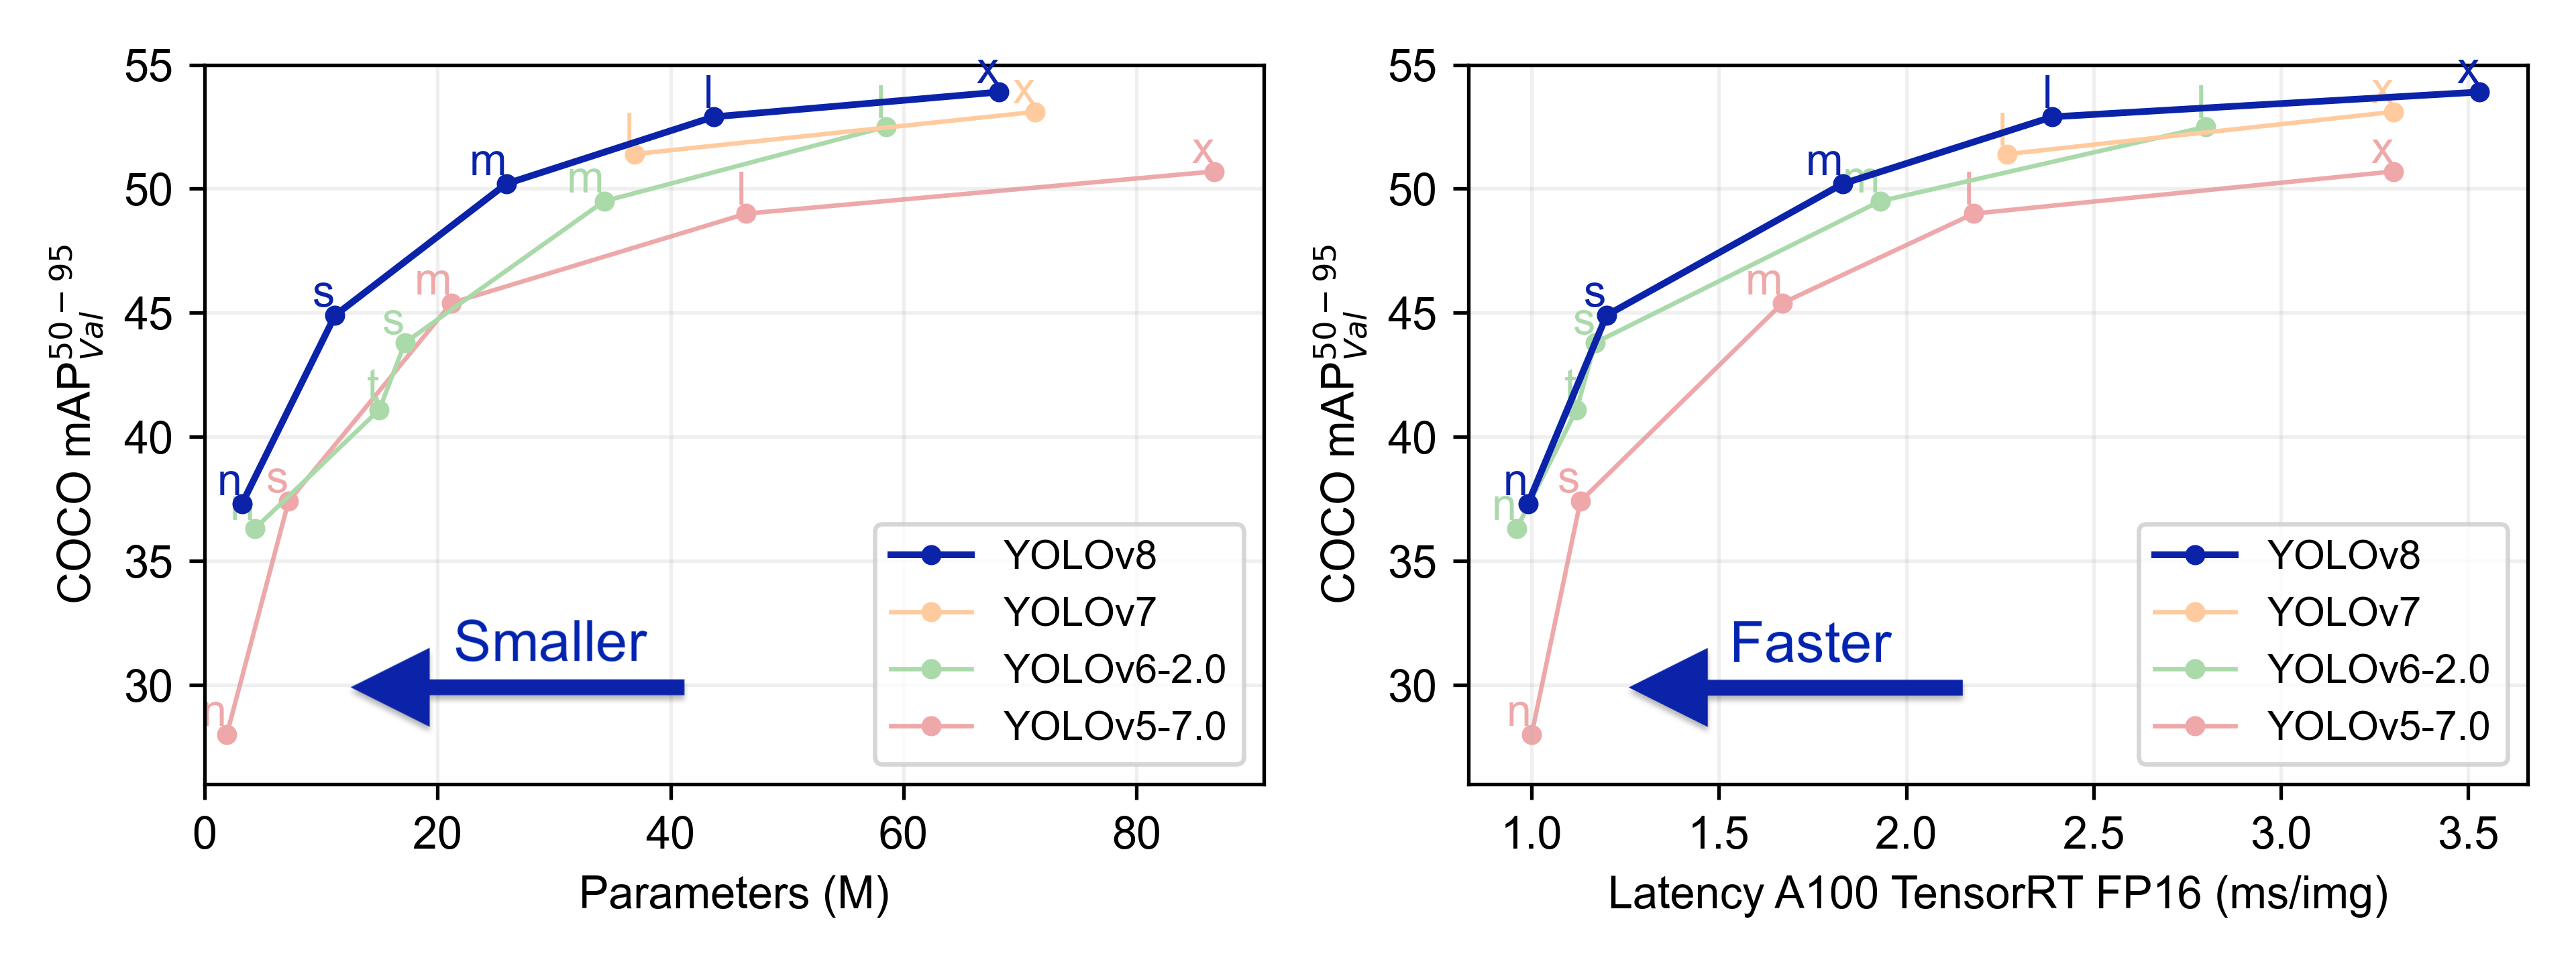
\includegraphics[width=0.95\textwidth]{images/4/YOLOVersiones.png}
    \caption{Rendimiento de diferentes versiones de \texttt{YOLO} superiores a la 5 en el conjunto de datos \texttt{COCO}\cite{ultralyticsYOLOv8}}
    \label{fig:YOLOVersiones}
\end{figure}

Esto ha convertido a \texttt{YOLO} en un estándar de facto en la implementación rápida de soluciones basadas en \texttt{Deep Learning} para muchos investigadores por sus resultados en la detección en tiempo real.

Actualmente \texttt{YOLO} es un proyecto llevado por la empresa \texttt{ultralytics}, siendo el último modelo \texttt{YOLOv8}. Este modelo está conformado por una capa convolucional personalizada basada en la 
arquitectura \texttt{CSPDarknet53}, que conecta diferentes fases convolucionales para obtener un entrenamiento mucho más rápido. Esta capa convolucional se conecta al cuello de \texttt{YOLO}, 
cuya función es utilizar varias salidas de algunas de las secciones de la capa convolucional para tener información de diferentes escalas (cada capa convolucional va transformando la anterior entrada en un vector más y más horizontal).

Lo anterior es común a todos los modelos de \texttt{YOLOv8} independientemente de la tarea que realizan, lo que cambia es la parte final de la red, que, aprovechando la presencia de datos de diferentes escalas, 
utiliza redes neuronales completamente conectadas para diferentes tareas, una para las localizaciones, otra para las probabilidades de clase de cada elemento y otra para trabajar con regiones de interés.

Para facilitar la lectura del documento, en el \hyperref[subsec:A]{anexo A} se realiza una explicación detallada de los parámetros e hiperparámetros habituales de los modelos de \texttt{YOLOv8}.


\subsubsection{Uso de redes neuronales en acuicultura}

La acuicultura es un trabajo que engloba desde la producción de algas hasta la crianza de marisco en cautiverio. Además, dentro de cada rama podemos tener especies que sean similares y que deban ser diferenciadas.

En la literatura de este ámbito se lleva implementando tecnologías basadas en aprendizaje automático para diferentes tareas, en el caso del uso de \texttt{\acrshort{cnn}} podemos ver sistemas para:
\begin{itemize}
    \item Sistemas de conteo de peces\cite{castillomoralSistemaConteoPeces2022}.
    \item Sistemas de análisis de densidad.
    \item Sistemas de seguimiento\cite{leeDetectionCatfishActivity2024}.
    \item Sistemas de diferenciación y detección de especies en entornos abiertos\cite{xiaSituSeaCucumber2018}\cite{ladeAutomatedFishSpecies2023}: aprovechando la existencia de conjuntos de datos
    \cite{ulucanLargeScaleDatasetFish2020} para experimentos con diferentes peces.
\end{itemize}

Existen ejemplos del uso de estas tecnologías en proyectos como el del \acrfullr{citsem} ``Acuicultura 4.0"\cite{Acuicultura} y diversos trabajos de fin de grado y máster relacionados, pero no para el conteo de movimientos a través de YOLO.

\clearpage
\subsection{Técnicas para el análisis de movimiento en la visión por ordenador}

Estas técnicas son muy importantes en el campo de la vigilancia, para poder percibir el cambio de elementos en la imagen y realizar su seguimiento. Según los autores M.Sonka y V.Hlavac\cite{sonkaImageProcessingAnalysis2013}, los problemas que 
trata se pueden dividir en tres grupos:

\begin{itemize}
    \item Detección de movimiento general, clasificando una imagen con o sin movimiento a través de un descriptor global.
    \item Detección y localización de objetos en movimiento, donde la escena es estática y el objeto se mueve sobre ella.
    \item Uso del movimiento para la reconstrucción 3D de una escena.
\end{itemize}

De los anteriores puntos, el más relevante en este trabajo es la detección y localización de objetos en movimiento (conteo de movimiento de un pez).

Debemos entender que el análisis de movimiento tiene en cuenta el eje temporal entre las imágenes, que puede tener muestras equiespaciadas o no. Es en este eje sobre el que queremos realizar el análisis, pero 
cabe destacar que hay muy poco análisis realizado sobre el uso de aprendizaje automático para estimación de movimiento en video. Los principales sistemas se basan en análisis a través de algoritmos.

\begin{itemize}
    \item \textbf{Análisis diferencial}: un ejemplo de esta técnica es la resta de una imagen número $n$ con la imagen número $n-1$, para obtener una diferencia en ciertos pixeles y determinar a través de un límite 
    la existencia de movimiento. Uno de los tipos de algoritmos más interesantes en este campo es el análisis de flujo óptico.
    \item \textbf{Correspondencia de puntos de interés}: se basa en la detección y seguimiento a través del eje temporal de ciertos puntos claves, para detectar el movimiento de elementos. Existen operadores para este 
    objetivo, pero no se adaptan bien a cambios demasiado rápidos.
    \item \textbf{Detección de patrones de movimiento}: uno de los pocos sistemas que se basa en entrenar un clasificador capaz de detectar patrones de movimiento, sin embargo son herramientas muy complejas 
    de implementar y tienen un alto coste computacional, ya que normalmente realizan las tres tareas: detección, clasificación y segmentación.
\end{itemize}

La mayoría de herramientas desarrolladas en este campo tienen necesidades muy específicas y no se adaptan bien a cambios demasiado bruscos, la única que puede manejarlos es una herramienta como el análisis de flujo óptico. 
Esto es debido a que se puede usar para analizar cambios entre todos los píxeles de las imágenes.

\subsubsection{Definición y uso del análisis de flujo óptico}

El análisis de flujo óptico u \texttt{OpticalFlow} apareció por primera vez en 1981\cite{hornDeterminingOpticalFlow1981} y se basa en asumir:

\begin{enumerate}
    \item El brillo observado en un punto del objeto es constante en el eje temporal.
    \item Puntos cercanos se mueven de la misma manera.
\end{enumerate}

El problema es que en las imágenes reales las reglas sobre el brillo y la suavidez del cambio es habitual que no sean respetadas. Esto puede ser por diversos motivos como poco \texttt{framerate} o movimientos 
muy cercanos a la cámara que generen cambios bruscos en los pixeles.

Es una técnica que se usa mucho en las carreteras, por la existencia de entornos muy estáticos. Se puede ver un ejemplo de su aplicación en la \autoref{fig:OpticalFlowEjemplo}.

\begin{figure}[H]
    \centering
    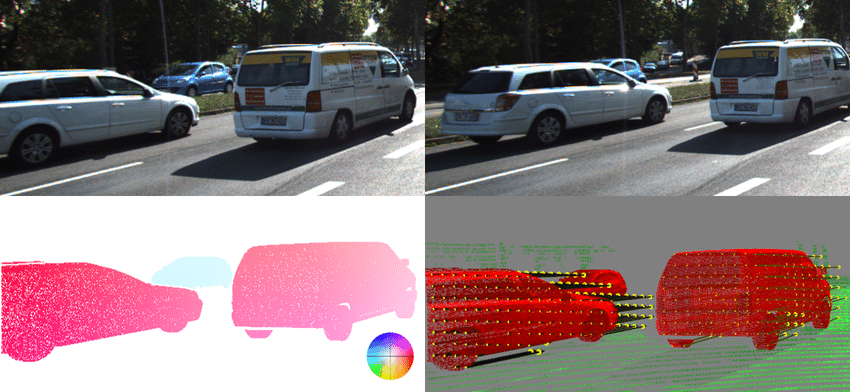
\includegraphics[width=0.8\textwidth]{images/4/OpticalFlow.png}
    \caption{Análisis del flujo óptico entre 2 fotogramas de una escena\cite{schusterCombiningStereoDisparity2018}}
    \label{fig:OpticalFlowEjemplo}
\end{figure}

Actualmente, existen tres algoritmos principales para calcular el flujo óptico de una escena:

\begin{itemize}
    \item Método Horn-Schunck: devuelve una estimación global.
    \item Método de Lucas-Kanade: asume que el flujo va a ser constante en los vecinos, y con esto, realiza una serie de estimaciones locales.
    \item Método combinado local-global: calcula el flujo óptico en zonas rectangulares de la imagen.
\end{itemize}

\subsubsection{Uso del análisis del flujo óptico en entornos de acuicultura}

El análisis de flujo óptico se ha usado en acuicultura de forma diversa:

\begin{itemize}
    \item Analizar comportamientos de grupo, por ejemplo, para determinar la actividad de un conjunto de peces de forma global\cite{kobayashiAquaColonyFully2023}.
    \item Realizar una detección, conteo y seguimiento de peces en un tanque en la India, mezclando \texttt{YOLOv5} con \texttt{OpticalFlow}\cite{paiComputerVisionBased2022}. Este método dio buenos resultados porque 
    la distancia del pez a la cámara era suficiente como para que no hubiese movimientos demasiado grandes como se puede ver en la \autoref{fig:DatosOpticalEstudio}.
\end{itemize}

\begin{figure}[H]
    \centering
    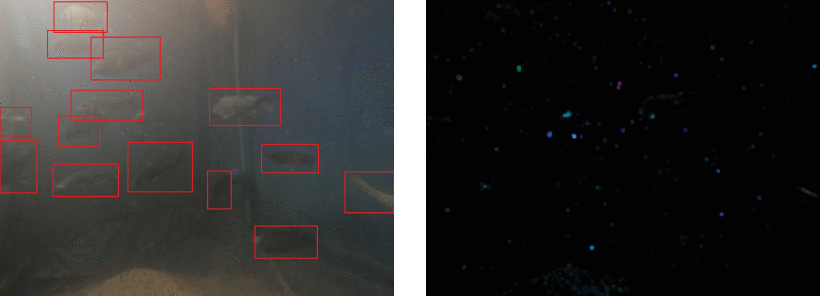
\includegraphics[width=0.9\textwidth]{images/4/OpticalFlowIndia.png}
    \caption{Datos obtenidos por OpticalFlow respetando las reglas de distancia sobre peces\cite{paiComputerVisionBased2022}}
    \label{fig:DatosOpticalEstudio}
\end{figure}
\clearpage


\subsection{Herramientas de desarrollo y despliegue en \texttt{HardWare} transparente}

\begin{itemize}
    \item \textbf{Librerías de desarrollo para Redes Neuronales}: Para trabajar en la creación de redes neuronales, se usan principalmente dos librerías: \texttt{Keras} y \texttt{PyTorch}.
    \texttt{Keras} es una librería de alto nivel, mientras que \texttt{PyTorch} es de bajo nivel y tiene mejores herramientas de manejo de errores y de control del rendimiento de la red creada. 
    Aparte de esto, \texttt{PyTorch} está pensado para su uso directamente en \texttt{Python} y soporta entrenamiento en sistemas distribuidos.


    En el caso de \texttt{YOLO}, la empresa \texttt{Ultralytics} retomó el proyecto y creo las versiones a partir de \texttt{YOLOv5}. El objetivo de esto ha sido crear una librería para 
    que el usuario no tenga que interactuar con las librerías de bajo nivel. Esto nos permite entrenar, validar y desplegar modelos a través de modelos base.
    \item \textbf{Transfer Learning y Fine Tunning}: Entrenar una red neuronal desde 0 es demasiado complejo, por ejemplo, una red \texttt{YOLOv8} de tamaño pequeño tiene \texttt{11.2} millones de pesos que 
    deben ser entrenados y ajustados. Estos pesos incluyen las capas convolucionales y la capa de clasificación.\newline
    Pero lo habitual es obtener un modelo ya entrenado, cuyas capas convolucionales sean capaces de extraer características típicas de cualquier imagen y, solo entrenar la parte de clasificación. 
    Esto reduce mucho el coste computacional de entrenamiento y por lo tanto, el tiempo requerido para llegar al objetivo deseado con la red. Esta técnica se conoce como \texttt{Transfer Learning} 
    y se puede ver en la \autoref{fig:TransferLearning}.
    
    \begin{figure}[H]
        \centering
        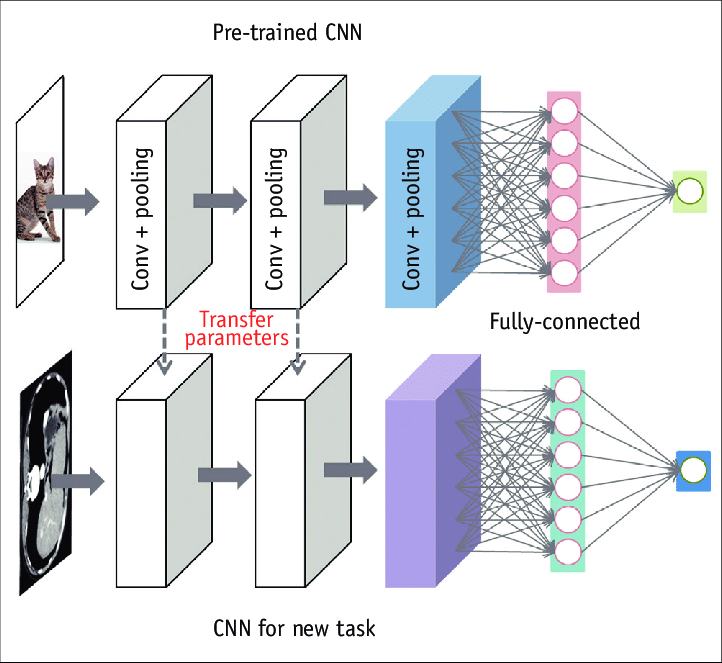
\includegraphics[width=0.65\textwidth]{images/4/TransferLearning.png}
        \caption{Uso de parámetros realizando \texttt{Transfer Learning}\cite{doBasicsDeepLearning2020}}
        \label{fig:TransferLearning}
    \end{figure}

    Posteriormente, cuando se alcanza el rendimiento esperado, se pueden desbloquear los pesos de las capas de convolución y hacer entrenamiento de toda la red. Esta fase se llama \texttt{Fine Tunning}. 
    Su objetivo es ajustar la capa de convolución también para solo analizar las características de la imagen más relevantes para la tarea.
    \item \textbf{Herramientas comunes para el análisis de flujo óptico}: En la mayoría de lenguajes existen librerías que implementan los algoritmos de análisis de flujo óptico, pero, al ser herramientas de 
    caracterización de imagen, existen muchas facilidades en entornos matemáticos como MATLAB o de procesado de datos como el lenguaje de programación \texttt{Python}, más concretamente la librería de \texttt{OpenCV}.
    
    \clearpage
    
    \item \textbf{Abstracción de la red neuronal al \texttt{HardWare}}: A la hora de desplegar una red neuronal, se debe diseñar una estrategia para 
    poder aprovechar todos los recursos del sistema que va a ejecutar la red. Esto es debido a que una red neuronal se aprovecha de la computación en paralelo, ya que principalmente 
    resuelve sumas y multiplicaciones con matrices.

    En este sentido, los despliegues más eficientes son los que son capaces de aprovechar elementos como las \texttt{\acrfullr{gpu}}, que se centran en este tipo de operaciones. Al contrario 
    que una \texttt{\acrfullr{cpu}}, la \texttt{\acrfullr{gpu}} cuenta con más núcleos de cómputo de menor potencia como se puede ver en la \autoref{fig:GPUCPU}.

    \begin{figure}[H]
        \centering
        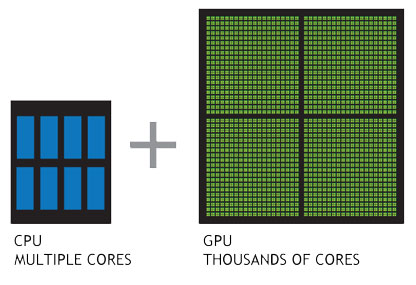
\includegraphics[width=0.5\textwidth]{images/4/GPUCores.jpg}
        \caption{Diferencia de cantidad de núcleos en una \texttt{CPU} y una \texttt{GPU}\cite{GPUVsCPU}}
        \label{fig:GPUCPU}
    \end{figure}

    En este sentido, según la plataforma de desarrollo de red neuronal que se utilice, el despliegue podrá aprovechar la gráfica dependiendo de factores como:
    
    \begin{itemize}
        \item Marca: \texttt{NVidia}, \texttt{AMD} o \texttt{Intel}.
        \item Generación del \texttt{HardWare}.
        \item Sistema Operativo en el que se despliega el sistema.
    \end{itemize}

    Por ejemplo, una red neuronal desarrollada en PyTorch solo soporta gráficas de \texttt{AMD} si el sistema operativo es \texttt{Linux}. Es por este motivo 
    que han surgido librerías abiertas que permiten el uso de una aceleración por \texttt{HardWare} común a muchos más dispositivos. Ejemplo de esto son los modelos 
    desarrollados en el entorno \texttt{ONNX}.
    De hecho, algunas empresas como \texttt{Intel} desarrollan sus propias librerías de herramientas para permitir compatibilidad con sus sistemas de aceleración. Estas librerías 
    suelen contener además, herramientas de transformación entre modelos para aportar más transparencia al usuario final y evitar problemas de compatibilidad.
\end{itemize}
